\documentclass[12pt, a4paper]{article}

% --- PAQUETES BÁSICOS ---
\usepackage[utf8]{inputenc}
\usepackage[spanish]{babel}
\usepackage[margin=2.5cm]{geometry}
\usepackage{graphicx}
\usepackage{amsmath}
\usepackage{hyperref}
\usepackage{tabularx} % Añadido para tablas auto-ajustables
\usepackage{array}    % Añadido para mejor formato en columnas

% --- CONFIGURACIÓN DE HIPERVÍNCULOS ---
\hypersetup{
    colorlinks=true,
    linkcolor=blue,
    filecolor=magenta,      
    urlcolor=cyan,
    pdftitle={Informe de Diseño: Brazo Robótico},
    pdfpagemode=FullScreen,
}

\title{\textbf{Informe de Diseño: Manipulador Robótico Móvil}}
\author{Nombre del Autor}
\date{\today}

\begin{document}

\maketitle
\thispagestyle{empty} 
\newpage

\pagenumbering{roman} 
\tableofcontents
\newpage

\pagenumbering{arabic} 

\section{Introducción y Contexto}

\subsection{Solicitud Inicial}
El proyecto nace como respuesta a un requerimiento interno del laboratorio para actualizar y expandir el equipamiento destinado a prácticas de robótica móvil. Se solicitó el diseño de un brazo manipulador de 4 grados de libertad (GdL) que fuera fácilmente acoplable a bases móviles existentes, priorizando el bajo costo de fabricación y la facilidad de mantenimiento frente al desgaste derivado del uso continuo por parte de los estudiantes.

\section{Parámetros de Diseño en Términos de Ingeniería}

\subsection{Restricciones}
\begin{itemize}
    \item \textbf{Limitación por Actuadores:} Las restricciones globales son dictaminadas por el torque máximo de los actuadores seleccionados. Este valor define directamente la longitud máxima viable de los eslabones, el payload, el alcance operativo, el tipo de herramientas intercambiables y los métodos de compensación de gravedad.
    \item \textbf{Materiales Estructurales:} La estructura está restringida a los insumos compatibles con la tecnología FDM de las impresoras 3D y maquinado CNC de la universidad. Esto limita la selección a termoplásticos como PLA, ABS, PETG y materiales maquinables.
\end{itemize}

\subsection{Entregables}
\begin{itemize}
    \item Manipulador Robótico Móvil ensamblado (4 GdL) modificable a (5 GdL).
    \item Controlador funcional implementado con microcontroladores.
    \item Código fuente documentado para el control del manipulador y cálculo cinemático.
    \item Conjunto de herramientas finales intercambiables.
    \item Manual de usuario, manual de mantenimiento, instrucciones de operación y consideraciones de seguridad.
    \item Planos, archivos CAD y lista de materiales (BOM).
\end{itemize}

\section{Definición del Proyecto}

\subsection{Necesidad}
\subsubsection{Estado Actual}
La robótica es un pilar fundamental en la actualidad, abarcando desde procesos de automatización industrial hasta aplicaciones de robótica móvil en diversos entornos, tales como exploración, manipulación en zonas inaccesibles, automatización de tareas pequeñas e investigación. Sin embargo, la accesibilidad y la asequibilidad de los manipuladores aún representan un desafío debido a factores como los altos costos de los brazos terminados, el precio elevado de ciertos servosistemas de calidad, la falta de capacitación y las limitaciones mecánicas y de precisión inherentes a los servosistemas de corriente directa de bajo coste. Por consiguiente, se presenta la necesidad de crear un prototipo de manipulador móvil robótico que sea personalizable, de fácil mantenimiento, de bajo coste y que ofrezca suficiente precisión y exactitud.

\subsubsection{Estado Deseado}
La solución propuesta que solventa esta necesidad corresponde a un prototipo de manipulador robótico tipo brazo articulado, con la posibilidad de ser acoplado a distintas plataformas móviles. Este manipulador debe poseer un alcance óptimo para la plataforma móvil.

\subsection{Requerimientos}

\textbf{Requerimientos Funcionales}
\begin{itemize}
    \item \textbf{Alcance espacial:} El manipulador debe poseer un alcance operativo radial apto para funcionar en la plataforma. 
    \item \textbf{Capacidad de carga (Payload):} El sistema debe manipular herramientas garantizando estabilidad.
    \item \textbf{Modularidad del efector final:} El extremo del brazo debe contar con una brida mecánica estandarizada para intercambiar rápidamente diversas herramientas.
    \item \textbf{Integración móvil:} El diseño de la base debe contemplar un patrón de anclaje estandarizado para instalación en plataformas móviles.
    \item \textbf{Control de trayectoria:} El algoritmo (interpolación espacial) y el hardware deben mitigar activamente el jitter y los sobreimpulsos dinámicos.
    \item \textbf{Precisión:} Movimientos fluidos con métricas de repetibilidad y exactitud que permitan tareas reales de agarre y coordenadas pre-programadas.
\end{itemize}

\textbf{Requerimientos No Funcionales y de Desempeño}
\begin{itemize}
    \item \textbf{Restricción presupuestal:} Uso intensivo de la metodología DIY y piezas COTS (Commercial Off-The-Shelf) para asegurar la viabilidad financiera del escalamiento (múltiples copias para el laboratorio).
    \item \textbf{Precisión y mitigación de Backlash:} El diseño de transmisión (o la selección directa del actuador) debe reducir mecánicamente el juego para evitar los errores espaciales de 2 a 7 mm evidenciados en iteraciones previas (Axum I).
    \item \textbf{Mantenibilidad:} Arquitectura mecánica enfocada en el fácil ensamblaje, cableado y conexiones.
\end{itemize}

\textbf{Requerimientos de Usuario y Entorno}
\begin{itemize}
    \item \textbf{Orientación pedagógica:} Código base comprensible, hardware expuesto pero seguro, y arquitectura abierta que invite a la modificación académica.
    \item \textbf{Escalabilidad:} El entorno de procesamiento debe contar con suficientes puertos y poder de cómputo remanente para futuras mejoras.
    \item \textbf{HMI (Interfaz Hombre-Máquina):} Integración de un sistema de operación intuitivo y visual, incluyendo paradas de emergencia por hardware y software.
\end{itemize}

\subsection{Parámetros de Diseño de Ingeniería}

\subsubsection{Análisis de Motores}
A partir de la revisión del estado del arte, se seleccionaron motores paso a paso bajo el estándar \textbf{NEMA 17}. Esta elección responde a las facilidades de intercambiabilidad que ofrece este estándar, la homologación de sus especificaciones eléctricas y mecánicas, y la disponibilidad de cajas de transmisión acoplables en el mercado.

Los motores seleccionados cuentan con un rotor de 50 polos y operan mediante tecnología híbrida, combinando las características de los motores de imán permanente con el principio de reluctancia variable. Si bien esta configuración optimiza su desempeño general, presenta ciertas ventajas y desventajas que deben ser contempladas en el diseño:

\paragraph{Desventajas}
\begin{itemize}
    \item \textbf{Inercia rotacional elevada:} Causada por la masa combinada del rotor de hierro y los imanes permanentes.
    \item \textbf{Relación masa-potencia:} Cuentan con un peso considerable frente a otras tecnologías de actuadores.
    \item \textbf{Dependencia magnética:} El rendimiento general está supeditado a la calidad e intensidad de la magnetización del rotor.
    \item \textbf{Sensibilidad térmica:} Su eficiencia y fuerza electromotriz se ven afectadas por incrementos en la temperatura de trabajo.
    \item \textbf{Caída de torque a altas velocidades:} El torque dinámico decae de forma no lineal a medida que se incrementa la frecuencia de pasos (velocidad de rotación).
\end{itemize}

\paragraph{Ventajas}
\begin{itemize}
    \item \textbf{Torque de remanencia (\textit{detent torque}):} Ofrecen una ligera retención mecánica incluso estando desenergizados.
    \item \textbf{Alta resolución y torque de sostenimiento (\textit{holding torque}):} Presentan una alta densidad de pasos por revolución y un torque estático configurable según la corriente suministrada.
    \item \textbf{Estabilidad dinámica:} Cuentan con un margen de resonancia significativamente más distante comparado con motores de reluctancia pura.
    \item \textbf{Escalabilidad dimensional:} Es posible incrementar el torque disponible aumentando únicamente la longitud axial del estator y rotor, manteniendo intactas la sección transversal y la brida de montaje NEMA 17.
\end{itemize}

En la Tabla~\ref{tab:control_stepper} se sintetizan las características principales de cada método de accionamiento. Se usa Tabularx para evitar desbordamientos.

\begin{table}[htbp]
\centering
\caption{Comparación de esquemas de excitación para motores paso a paso NEMA 17.}
\label{tab:control_stepper}
\begin{tabularx}{\textwidth}{|>{\raggedright\arraybackslash}p{2.5cm}|>{\raggedright\arraybackslash}X|>{\raggedright\arraybackslash}X|>{\raggedright\arraybackslash}X|}
\hline
\textbf{Parámetro} & \textbf{Paso Completo (1 Fase)} & \textbf{Paso Completo (2 Fases)} & \textbf{Micropaso (\textit{Microstepping})} \\ \hline
\textbf{Excitación} & Una bobina energizada por paso. & Dos bobinas energizadas simultáneamente. & Modulación de corriente seno/coseno en ambas bobinas. \\ \hline
\textbf{Resolución} & Base (ej. $1.8^\circ$ / paso o 200 pasos/rev). & Base (ej. $1.8^\circ$ / paso), desplazado $0.9^\circ$. & Altamente incrementada (ej. $1/16$, $1/32$ hasta $1/256$ de paso). \\ \hline
\textbf{Suavidad y Ruido} & Baja; alta vibración por resonancia. & Intermedia; presenta rizado dinámico. & Elevada; movimiento continuo y silencioso. \\ \hline
\textbf{Torque de Salida} & Bajo ($\sim 70\%$ del nominal). & Máximo torque estático ($100\%$ nominal). & Torque dinámico suave, pero menor torque incremental por micropaso. \\ \hline
\textbf{Lógica de Control} & Lógica binaria elemental (Secuencia en anillo). & Lógica binaria elemental (Secuencia en anillo). & Requiere modulación por ancho de pulso (PWM) y control de corriente. \\ \hline
\end{tabularx}
\end{table}

\paragraph{Caracterización Técnica y Dimensional del Estándar NEMA 17}
El estándar \textbf{NEMA 17} define principalmente las dimensiones del plato de montaje frontal ($42.3 \times 42.3\text{ mm}$). Los parámetros representativos se detallan en la Tabla~\ref{tab:nema17_specs}.

\begin{table}[htbp]
\centering
\caption{Especificaciones mecánicas y eléctricas representativas de un motor NEMA 17 típico.}
\label{tab:nema17_specs}
\begin{tabularx}{\textwidth}{|l|l|>{\raggedright\arraybackslash}X|}
\hline
\textbf{Categoría} & \textbf{Parámetro} & \textbf{Valor Típico / Rango} \\ \hline
\textbf{Mecánica} & Dimensiones del marco & $42.3\text{ mm} \times 42.3\text{ mm}$ (NEMA 17) \\ \hline
 & Longitud del cuerpo ($L$) & $34\text{ mm} - 48\text{ mm}$ (depende del torque nominal) \\ \hline
 & Diámetro del eje (\textit{Shaft}) & $\phi\,5.0\text{ mm}$ (frecuentemente con plano D-cut) \\ \hline
 & Longitud sobresaliente del eje & $20\text{ mm} - 24\text{ mm}$ \\ \hline
 & Patrón de montura & 4 agujeros M3 $\times 0.5$ (profundidad $\sim 4.5\text{ mm}$) \\ \hline
 & Masa del motor & $280\text{ g} - 500\text{ g}$ \\ \hline
\textbf{Eléctrica} & Configuración de fases & Bipolar (4 hilos) / Unipolar (6 hilos) \\ \hline
 & Corriente nominal por fase & $1.2\text{ A} - 1.8\text{ A}$ RMS \\ \hline
 & Resistencia por fase & $1.5\,\Omega - 3.3\,\Omega$ \\ \hline
 & Inductancia por fase & $2.8\text{ mH} - 8.0\text{ mH}$ \\ \hline
\textbf{Magnética} & Ángulo de paso nativo & $1.8^\circ \pm 5\%$ (200 pasos/rev) \\ \hline
 & Torque de sostén (\textit{Holding}) & $20\text{ N}\cdot\text{cm} - 80\text{ N}\cdot\text{cm}$ ($0.40 - 0.55\text{ N}\cdot\text{m}$) \\ \hline
 & Inercia del rotor & $54\text{ g}\cdot\text{cm}^2 - 68\text{ g}\cdot\text{cm}^2$ \\ \hline
\end{tabularx}
\end{table}

\paragraph{Análisis de Torques en Motores Paso a Paso}
Para el diseño mecatrónico y la validación de las trayectorias del manipulador, es indispensable analizar los diferentes regímenes de par mecánico que presenta un actuador paso a paso.

\begin{description}
    \item[\textbf{Torque de Mantenimiento (\textit{Holding Torque}, $T_H$):}] Es el par estático máximo.
    \item[\textbf{Torque de Detención (\textit{Detent Torque}, $T_D$):}] Es el par de retención residual cuando el motor no está energizado.
    \item[\textbf{Torque de Arranque (\textit{Pull-in Torque}):}] Es el par dinámico máximo de arranque instantáneo.
    \item[\textbf{Torque de Desplazamiento (\textit{Pull-out Torque}):}] Límite absoluto de par dinámico.
    \item[\textbf{Rango de Aceleración (\textit{Slew Range}):}] Región operativa entre Pull-in y Pull-out.
\end{description}

\begin{figure}[htbp]
    \centering
    % Se mantiene la opción draft para que compile sin la imagen
    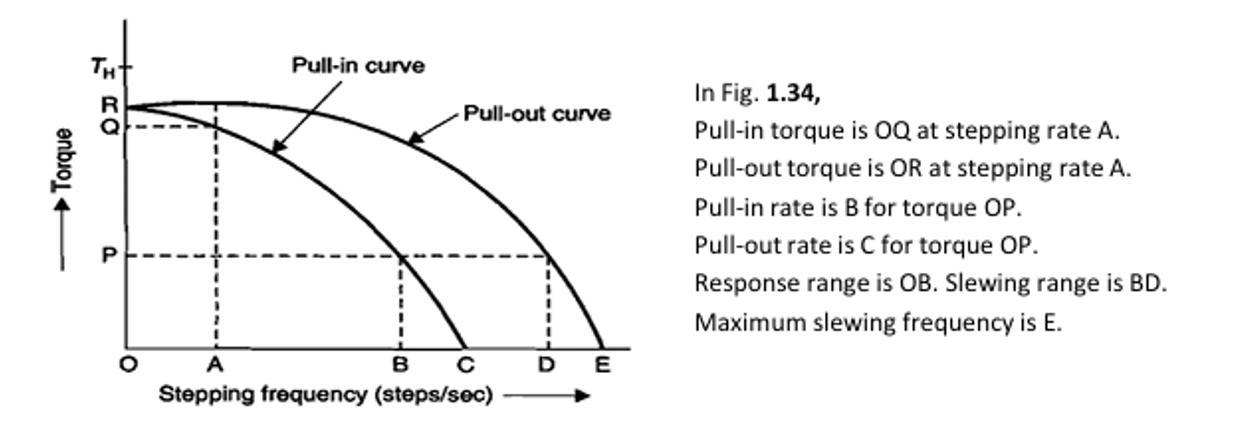
\includegraphics[width=0.8\textwidth]{T_in_out.png}
    \caption{Curvas características de par dinámico frente a la frecuencia de pasos.}
    \label{fig:torque_stepper}
\end{figure}

\paragraph{Dinámica de Corriente Limitada por Voltaje}
El torque a altas velocidades decae porque la inductancia y la FCEM impiden que la corriente alcance el valor nominal $I_{ph}$.
\begin{equation}
    I_{env}(\omega_m) = \frac{V - K_t \omega_m}{\sqrt{R^2 + (N_r \omega_m L)^2}}
\end{equation}

\subsubsection{Análisis Cinético y Dinámica Inversa}
El modelo dinámico del manipulador evalúa los torques requeridos en cada articulación para vencer la gravedad y las fuerzas inerciales durante una trayectoria. 

\begin{equation}
    \tau_{g,i} = \left| \sum_{j=i}^{n} \left( \mathbf{r}_{L,j} \times m_{L,j} \mathbf{g} \right) + \sum_{k \in \{mot \ge i\}} \left( \mathbf{r}_{mot,k} \times m_{mot,k} \mathbf{g} \right) + \left( \mathbf{r}_{tip} \times m_{tip} \mathbf{g} \right) \right| \cdot \mathbf{z}_i
\end{equation}

\paragraph{Propagación del Error Espacial por Backlash}
Las cajas reductoras mecánicas introducen inherentemente un juego mecánico o \textit{backlash} angular ($\Delta\theta$) en cada articulación.
\begin{equation}
    \Delta\mathbf{p} \approx \mathbf{J}(\mathbf{\Theta}) \cdot \Delta\mathbf{\Theta}
\end{equation}

\textbf{Mapeo de Incertidumbre y Envolvente Convexa (\textit{Convex Hull}):} 
Dado que cada transmisión posee un error angular independiente acotado en el intervalo $[-\Delta\theta_{max}, +\Delta\theta_{max}]$, la posición real del efector final no converge en un punto único, sino dentro de un volumen de incertidumbre.

\subsubsection{Parámetros de Motores y Transmisiones Seleccionados}
Los parámetros electromecánicos nominales de los motores base seleccionados se consolidan en el Cuadro~\ref{tab:motores_seleccionados}:

\begin{table}[htbp]
\centering
\caption{Especificaciones nominales de los motores paso a paso NEMA 17 seleccionados.}
\label{tab:motores_seleccionados}
\resizebox{\textwidth}{!}{%
\begin{tabular}{|l|c|c|c|c|}
\hline
\textbf{Parámetro} & \textbf{17HD60001-22B} & \textbf{Motor Serie TS} & \textbf{17HS4401} & \textbf{17HS08-1004S} \\ 
 & \textit{(Alta Potencia)} & \textit{(Base TS4215)} & \textit{(Estándar)} & \textit{(Pancake)} \\ \hline
\textbf{Corriente Nominal ($I_{ph}$)} & 1.5 A & 1.7 A & 1.5 A & 1.0 A \\ \hline
\textbf{Resistencia de Fase} & $2.4\,\Omega \pm 10\%$ & $1.5\,\Omega \pm 10\%$ & $1.5\,\Omega \pm 10\%$ & $3.5\,\Omega \pm 10\%$ \\ \hline
\textbf{Inductancia de Fase} & 5.0 mH $\pm 20\%$ & 2.8 mH $\pm 20\%$ & 2.8 mH $\pm 20\%$ & 4.5 mH $\pm 20\%$ \\ \hline
\textbf{Holding Torque ($T_H$)} & 65 N$\cdot$cm & 42 N$\cdot$cm & 42 N$\cdot$cm & 16 N$\cdot$cm \\ \hline
\textbf{Inercia del Rotor ($J_m$)} & 102 g$\cdot$cm$^2$ & 54 g$\cdot$cm$^2$ & 54 g$\cdot$cm$^2$ & 22 g$\cdot$cm$^2$ \\ \hline
\textbf{Masa Total} & $\sim$500 g & $\sim$280 g & $\sim$280 g & $\sim$150 g \\ \hline
\end{tabular}%
}
\end{table}

\subsubsection{Cálculos de Motores y Transmisiones Seleccionados}

Para comparar los motores y como afectan las perdidas se crearon las siguientes graficas
\begin{figure}[htbp]
    \centering
    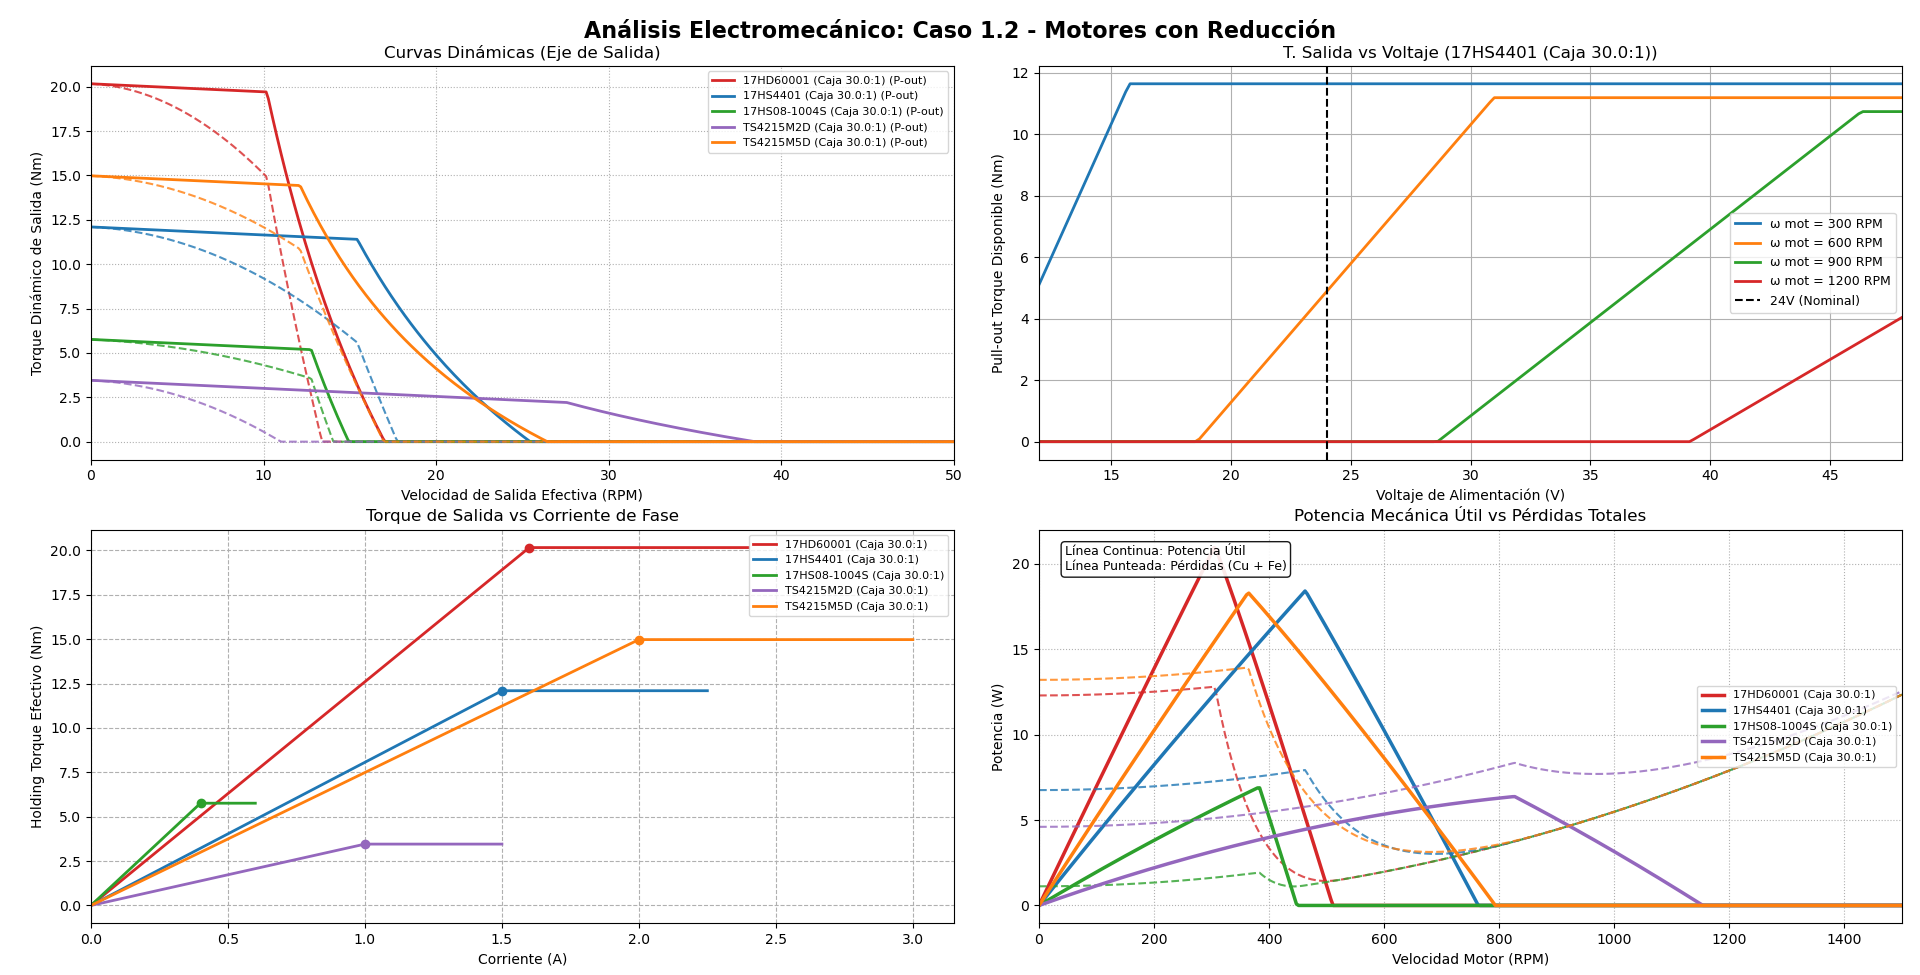
\includegraphics[ width=0.9\textwidth]{Tvsw_30_1.png}
    \caption{Curvas dinámicas (Pull-out y Pull-in) y balance de potencias.}
    \label{fig:curvas_dinamicas_30_1}
\end{figure}

\begin{figure}[htbp]
    \centering
    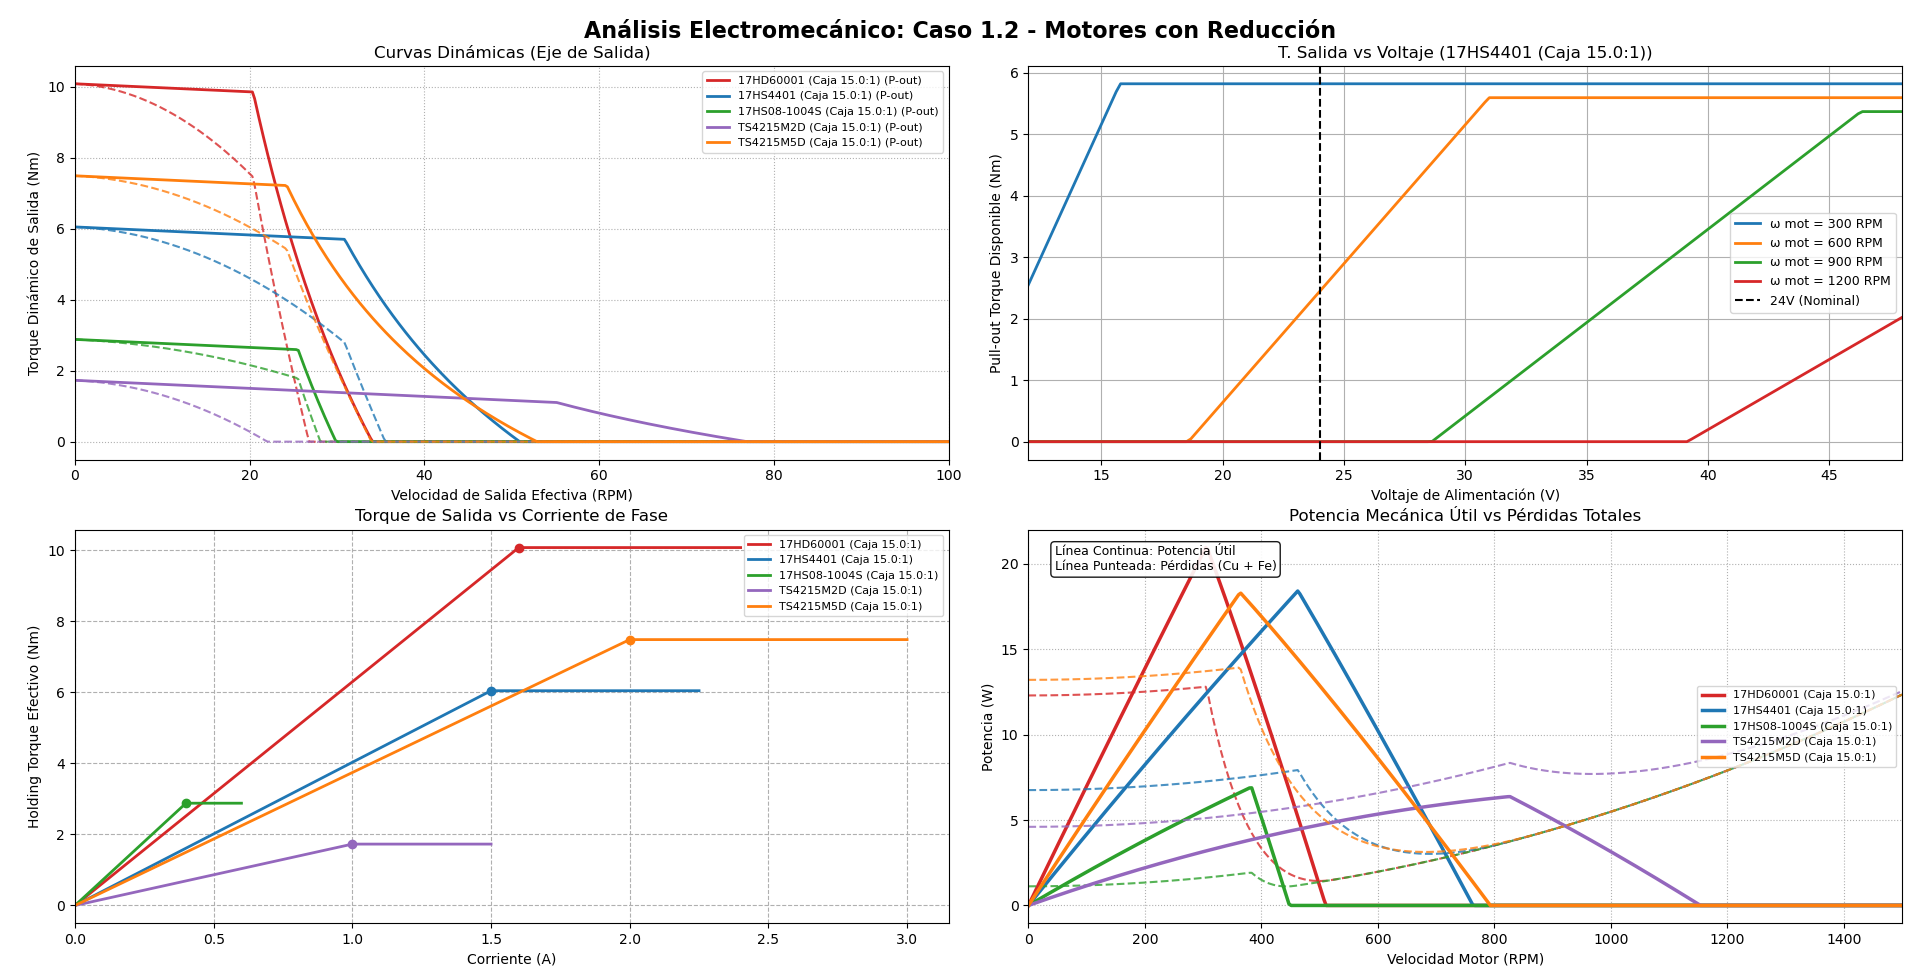
\includegraphics[ width=0.9\textwidth]{Tvsw_15_1.png}
    \caption{Curvas dinámicas (Pull-out y Pull-in) y balance de potencias.}
    \label{fig:curvas_dinamicas_30_1}
\end{figure}



Para validar la viabilidad del diseño estructural bajo distintas longitudes focales, se simuló el escalamiento del brazo empleando motores paso a paso de la serie TS4230.
\begin{figure}[htbp]
    \centering
    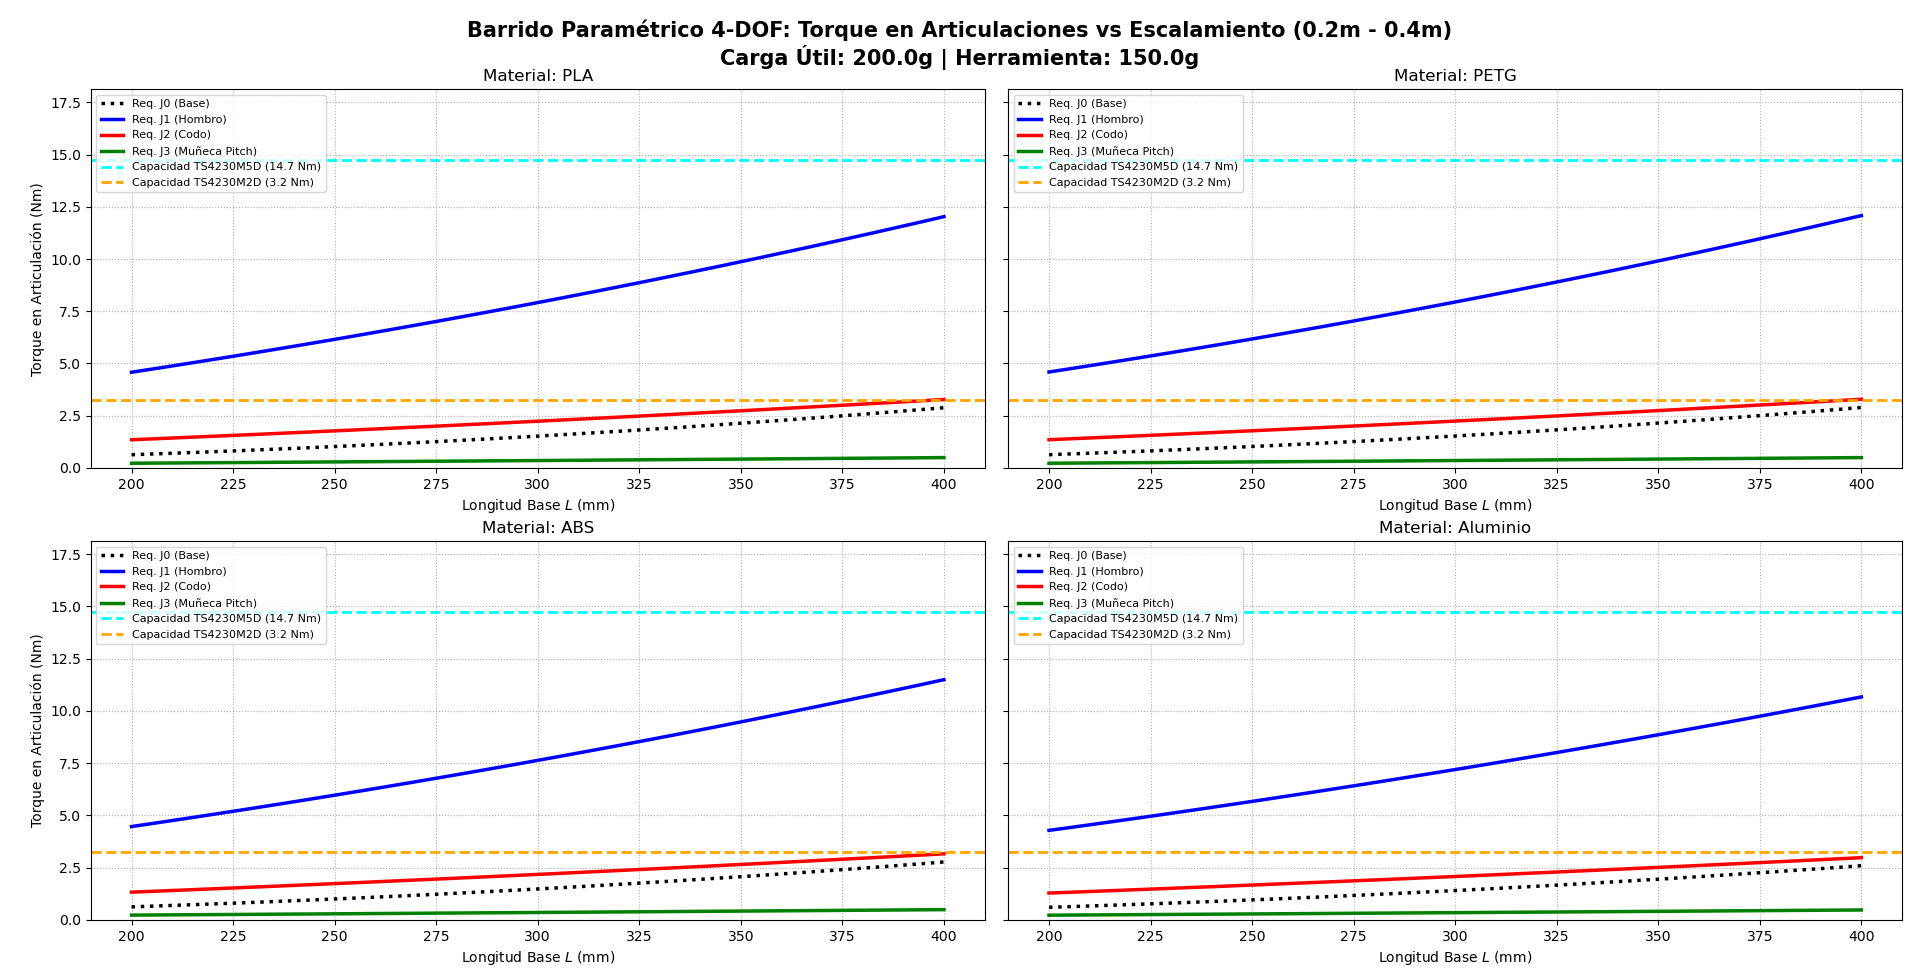
\includegraphics[ width=\textwidth]{TvsL4gof.png}
    \caption{Barrido paramétrico (4-DOF): Requerimiento de torque en articulaciones.}
    \label{fig:barrido_4dof}
\end{figure}

\begin{figure}[htbp]
    \centering
    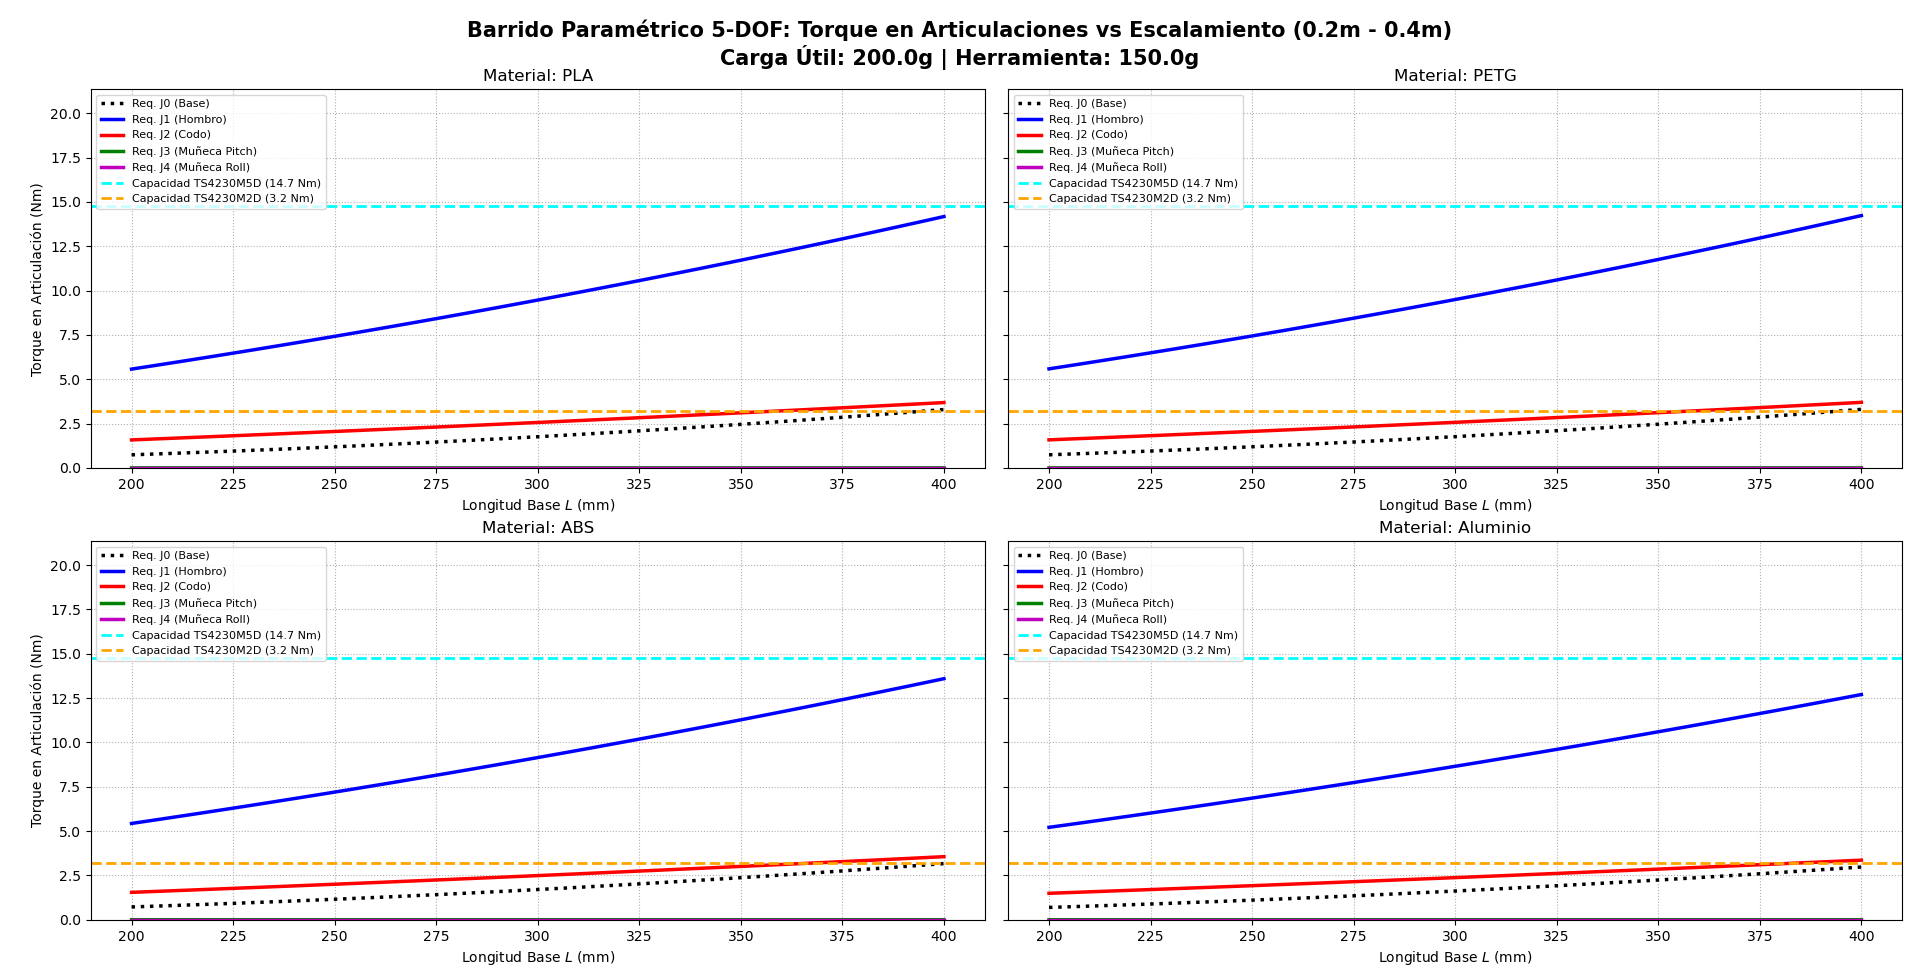
\includegraphics[ width=\textwidth]{TvsL5gof.png}
    \caption{Barrido paramétrico (5-DOF): Requerimiento de torque incluyendo el eje de rotación de muñeca.}
    \label{fig:barrido_5dof}
\end{figure}

Las Figuras \ref{fig:barrido_4dof} y \ref{fig:barrido_5dof} demuestran cómo la densidad del material incrementa drásticamente las inercias distales. 



\end{document}